\chapter{Dai rendimenti al grafo dinamico}
\label{ch:dynamic-correlation-graph}

I capitoli precedenti hanno costruito la matematica dei grafi e i modelli che apprendono dai dati, assumendo questi ultimi disponibili sotto forma di segnale sui nodi e di matrice dei pesi. A partire da questo capitolo si colma la distanza tra tali assunzioni e il caso di studio reale, affiancando alla teoria, qualora la pipeline di \texttt{cryptognn} ne offrisse un riscontro diretto, il frammento di codice che la realizza, seguendo l'ordine in cui essa genera i propri artefatti.

\section{L'universo cripto}
\label{sec:crypto-universe}

Lo studio segue quindici criptovalute quotate contro USDT su Binance: Bitcoin (BTC), Ethereum (ETH), BNB, XRP, Cardano (ADA), Solana (SOL), Dogecoin (DOGE), Polkadot (DOT), Avalanche (AVAX), Chainlink (LINK), Litecoin (LTC), Bitcoin Cash (BCH), Stellar (XLM), TRON (TRX) ed Ethereum Classic (ETC).

Il criterio di selezione è duplice. Ogni asset deve essere quotato con continuità su Binance da dicembre 2020, mese immediatamente precedente all'inizio del periodo di studio, in modo che nessuna serie presenti osservazioni mancanti all'interno della finestra osservata.
Nessun asset selezionato è inoltre una stablecoin. Il prezzo di una stablecoin oscilla per costruzione pochissimo attorno al valore ancorato. Una serie di questo tipo avrebbe quindi correlazione quasi nulla con il resto dell'universo e comparirebbe nel grafo come un nodo isolato che non porta informazione.

Il primo criterio introduce un survivorship bias esplicito: un asset collassato nel corso del periodo non può, per costruzione, soddisfarlo, indipendentemente dalla sua rilevanza per il mercato. È il caso di Terra/Luna, il cui collasso nel maggio 2022 è già stato richiamato nell'Introduzione come una delle tre crisi di riferimento dello studio. La struttura di correlazione che il \cref{ch:topological-evolution} misura in corrispondenza di quell'evento riguarda dunque la reazione degli altri asset dell'universo, non l'asset all'origine della crisi, escluso per costruzione dal campione.

Il periodo di studio copre l'intervallo dal 1\textsuperscript{o} gennaio 2021 al 30 giugno 2026, con osservazioni giornaliere chiuse convenzionalmente a mezzanotte UTC. Tale ampiezza include i tre eventi di crisi — la stretta cinese su scambi e mining nel maggio 2021, il collasso di Terra/Luna nel maggio 2022 e il fallimento di FTX nel novembre 2022 — con un margine consistente di osservazioni precedenti a ciascuna.

\subsection{Formato OHLCV e array posizionali}
\label{sec:ohlcv-positional-arrays}

Il progetto acquisisce i dati interrogando direttamente l'endpoint pubblico REST di Binance \path{/api/v3/klines}. Ogni chiamata GET specifica il simbolo della coppia di trading, ovvero la concatenazione del simbolo dell'asset e di quello della valuta di quotazione (es. \texttt{BTC} + \texttt{USDT} = \texttt{BTCUSDT}), l'intervallo di aggregazione delle candele e l'istante di inizio della richiesta.

Una candela riassume l'attività di prezzo di un asset in un intervallo di tempo fissato, che nel caso di studio coincide con un giorno, attraverso quattro valori (\cref{fig:candlestick}): il prezzo di apertura e di chiusura dell'intervallo, delimitati dal corpo della candela, il massimo e il minimo toccati al suo interno, rappresentati dalle estremità dello stoppino. Il colore del corpo segnala il segno della variazione, verde se il prezzo di chiusura supera quello di apertura (mercato rialzista), rosso in caso contrario (mercato ribassista).

\begin{figure}[H]
\centering
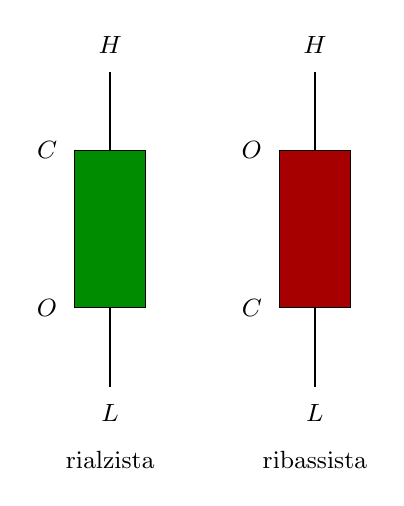
\begin{tikzpicture}[every node/.style={font=\small}]
    % candela verde (rialzista)
    \draw[thick] (0,0) -- (0,4);
    \filldraw[fill=green!55!black, draw=black] (-0.45,1) rectangle (0.45,3);
    \node[left] at (-0.55,1) {$O$};
    \node[left] at (-0.55,3) {$C$};
    \node[above] at (0,4.1) {$H$};
    \node[below] at (0,-0.1) {$L$};
    \node[below] at (0,-0.7) {rialzista};

    % candela rossa (ribassista)
    \begin{scope}[xshift=2.6cm]
        \draw[thick] (0,0) -- (0,4);
        \filldraw[fill=red!65!black, draw=black] (-0.45,1) rectangle (0.45,3);
        \node[left] at (-0.55,3) {$O$};
        \node[left] at (-0.55,1) {$C$};
        \node[above] at (0,4.1) {$H$};
        \node[below] at (0,-0.1) {$L$};
        \node[below] at (0,-0.7) {ribassista};
    \end{scope}
\end{tikzpicture}
\caption[Candela OHLC]{Rappresentazione di una candela giornaliera. Il corpo delimita apertura ($O$) e chiusura ($C$), lo stoppino il massimo ($H$) e il minimo ($L$) toccati nell'intervallo. Il colore segnala il segno della variazione: verde se $C>O$, rosso se $C<O$.}
\label{fig:candlestick}
\end{figure}

Binance restituisce al più $1\,000$ candele per chiamata, una per ciascun intervallo temporale coperto~\cite{binance_api_docs}. La risposta non è tuttavia una sequenza di oggetti con campi nominati, ma un array JSON di array posizionali: in Binance, ogni candela è rappresentata da una lista di dodici valori, la cui interpretazione dipende esclusivamente dalla posizione e non da un nome di campo. L'ordine documentato dall'exchange non è reso esplicito da alcuna struttura dati, e la ricostruzione di un DataFrame risulta pertanto complessa. Il caso di studio ovvia al problema definendo una lista \texttt{\_KLINE\_COLUMNS} dei dodici nomi di campo nello stesso ordine restituito dall'API, impiegata per etichettare le colonne del DataFrame contestualmente alla sua costruzione (\cref{lst:kline-columns}).

\begin{listing}[H]
\begin{minted}{python}
_KLINE_COLUMNS = [
    "open_time",
    "open",
    "high",
    "low",
    "close",
    "volume",
    "close_time",
    "quote_volume",
    "trades",
    "taker_buy_base",
    "taker_buy_quote",
    "ignore",
]
\end{minted}
\caption{\texttt{\_KLINE\_COLUMNS}}
\label{lst:kline-columns}
\end{listing}

I campi relativi al prezzo di apertura (\texttt{open}), al massimo (\texttt{high}), al minimo (\texttt{low}), al prezzo di chiusura (\texttt{close}) e al volume (\texttt{volume}), inteso come la quantità dell'asset scambiata nel periodo considerato, corrispondono all'acronimo OHLCV.

I rimanenti sette comprendono gli istanti di apertura e di chiusura della candela (\texttt{open\_time}, \texttt{close\_time}), il volume espresso nella valuta di quotazione anziché nell'asset base (\texttt{quote\_volume}), il numero totale di operazioni eseguite nell'intervallo (\texttt{trades}) e la quota di quel volume dovuta ad acquisti aggressivi, cioè eseguiti a mercato invece che tramite un ordine in attesa, espressa rispettivamente nell'asset base (\texttt{taker\_buy\_base}) e nella valuta di quotazione (\texttt{taker\_buy\_quote}). Il dodicesimo è un campo residuo, storicamente a uso interno di Binance (\texttt{ignore}, tipicamente nullo). Non tutti questi campi sono mantenuti in fase di costruzione del DataFrame.

\subsection{Paginazione e cache su disco}
\label{sec:pagination-disk-cache}

Una singola chiamata GET risulta insufficiente a coprire l'intero periodo di studio: il limite di $1\,000$ candele per risposta risulta infatti sensibilmente inferiore ai $2\,007$ giorni compresi tra il 1\textsuperscript{o} gennaio 2021 e il 30 giugno 2026. Il progetto provvede pertanto a suddividere le chiamate in pagine successive. Al termine di ciascuna risposta, viene rilevato l'istante di apertura dell'ultima candela ricevuta, a partire dal quale viene predisposta la chiamata successiva; il ciclo si ripete fino al raggiungimento dell'istante di fine richiesto (\cref{lst:pagination-loop}).

\begin{listing}[H]
\begin{minted}{python}
while True:
    batch = _fetch_klines_batch(symbol, interval, current_start, limit=limit)
    if not batch:
        break
    all_klines.extend(batch)
    last_open_time = batch[-1][0]
    if last_open_time >= end_time_ms:
        break
    current_start = last_open_time + 1
    time.sleep(0.15)
\end{minted}
\caption{\texttt{\_fetch\_klines\_paginated}}
\label{lst:pagination-loop}
\end{listing}

Prima di interrogare Binance, il progetto verifica se una cache locale copra già l'intervallo richiesto; in caso affermativo, i dati già presenti su disco vengono restituiti direttamente, senza alcuna chiamata di rete. Tale meccanismo conferisce idempotenza alle esecuzioni ripetute della pipeline: il rilancio dello script di download, qualora i dati siano già stati acquisiti, comporta unicamente la lettura di un file (\cref{lst:disk-cache-lookup}), salvo che non venga esplicitamente richiesto un nuovo download completo (flag \path{--force}).

\begin{listing}[H]
\begin{minted}{python}
if not force and cache_path.exists():
    cached = pd.read_parquet(cache_path)
    if cached.index.min() <= start_ts and cached.index.max() >= end_ts:
        return cached.loc[start_ts:end_ts]
\end{minted}
\caption{\texttt{fetch\_klines}}
\label{lst:disk-cache-lookup}
\end{listing}

La procedura sin qui descritta consente il download di un singolo asset. Una funzione di livello superiore ne ripete l'esecuzione sui quindici simboli che compongono l'universo di riferimento, mentre lo script \path{01_download_data.py} costituisce l'effettivo punto di ingresso, eseguito allo scopo di popolare la directory \path{data/raw/} con un file Parquet per ciascun asset.

Dei dodici campi restituiti da Binance, soltanto quattro vengono conservati come colonne del DataFrame scritto su disco: \texttt{close}, \texttt{volume}, \texttt{quote\_volume} e \texttt{trades}. A questi si aggiunge l'istante di apertura, impiegato però come indice del DataFrame anziché come colonna. Il dettaglio più rilevante è che, nonostante la candela sia descritta da quattro prezzi (\cref{fig:candlestick}), solamente il valore $C$ viene mantenuto, poiché lo studio calcola i rendimenti da chiusura a chiusura (\cref{sec:returns-stationarity}). Gli ulteriori campi esclusi, l'istante di chiusura, i due campi relativi agli acquisti aggressivi e il campo residuo privo di significato informativo, non trovano impiego in nessuna fase successiva dello studio.

\section{La serie temporale dei rendimenti}
\label{sec:returns-stationarity}

Tra i campi conservati dalla pipeline (\cref{sec:pagination-disk-cache}), questa sezione lavora sul prezzo di chiusura $P_t$ di ciascun asset, dato grezzo su cui si basa l'elaborazione successiva. Non si tratta, però, della quantità su cui si costruiscono i modelli. Due motivazioni ne inibiscono l'utilizzo.

La prima riguarda la scala. Una variazione assoluta di \$100 produce un impatto percentuale diverso a seconda che sia riferita ad un asset con un valore nominale di \$200 rispetto ad uno di \$60\,000. Ne consegue che il confronto diretto delle variazioni di prezzo tra asset diversi non è matematicamente informativo.

La seconda è la stazionarietà. Una serie temporale $\{x_t\}$ si dice stazionaria in senso debole (o stazionaria in media e varianza) se il valore atteso, la varianza e la funzione di autocovarianza $\mathrm{Cov}(x_t, x_{t+h})$ risultano invarianti rispetto al tempo $t$, dipendendo esclusivamente dal ritardo $h$
$$\mathbb{E}[x_t] = \mu, \quad \mathrm{Var}(x_t) = \sigma^2, \quad \mathrm{Cov}(x_t, x_{t+h}) = \gamma(h).$$
La serie dei prezzi $\{P_t\}$ non soddisfa il requisito di stazionarietà. Formalizzando il processo come un cammino aleatorio privo di deriva
$$P_t = P_{t-1} + \varepsilon_t, \quad \text{con } \mathbb{E}[\varepsilon_t] = 0 \text{ e } \mathrm{Var}(\varepsilon_t) = \sigma^2,$$
la varianza incondizionata al tempo $t$ è pari a
$$\mathrm{Var}(P_t) = t\sigma^2.$$
La dipendenza lineare della varianza da $t$ implica un'espansione indefinita della dispersione al procedere del tempo, violando la condizione di stazionarietà. Applicando l'operatore di differenza al logaritmo dei prezzi, come nell'equazione~\eqref{eq:price-returns}, si ottiene una serie trasformata a varianza costante nel tempo.

Per queste ragioni, la modellistica finanziaria adotta la serie dei rendimenti anziché quella dei prezzi, articolata nelle due principali varianti operative:
\begin{equation}
\label{eq:price-returns}
\begin{array}{c}
R_t = \dfrac{P_t - P_{t-1}}{P_{t-1}} \\[4pt]
\text{\footnotesize Rendimento semplice}
\end{array}
\qquad
\begin{array}{c}
r_t = \log\dfrac{P_t}{P_{t-1}} = \log P_t - \log P_{t-1} \\[4pt]
\text{\footnotesize Rendimento logaritmico}
\end{array}.
\end{equation}

La pipeline lavora con i log-rendimenti $r_t$ in fase di modellazione, riservando i rendimenti semplici $R_t$ al solo backtest (\cref{ch:backtest}), per tre motivi concreti:
\begin{enumerate}
\item \emph{Additività temporale}. Il log-rendimento cumulato su $k$ periodi equivale alla somma lineare $r_{t-k+1}+\dots+r_t$ dei singoli rendimenti di periodo. Al contrario, l'aggregazione temporale dei rendimenti semplici richiede la produttoria $\prod_{i=0}^{k-1} (1 + R_{t-i})$, introducendo una non linearità nella struttura del modello.
\item \emph{Simmetria di scala}. Una variazione di prezzo che raddoppia o dimezza il valore dell'asset genera rendimenti simmetrici pari a $\pm\log(2) \approx \pm0{,}693$. In termini di rendimenti semplici, i medesimi eventi producono invece una risposta asimmetrica pari a $+100\%$ e $-50\%$, introducendo distorsioni sistematiche nella stima dei momenti campionari e delle matrici di correlazione.
\item \emph{Approssimazione asintotica}. Per variazioni percentuali di modesta entità, i log-rendimenti costituiscono un'approssimazione al primo ordine dei rendimenti semplici. Dallo sviluppo in serie di Taylor della funzione $\log(1 + R_t)$ nell'intorno di $R_t = 0$:
$$r_t = \log(1 + R_t) = R_t - \frac{R_t^2}{2} + \frac{R_t^3}{3} - O(R_t^4)$$
si deduce che $r_t \approx R_t$ con un errore di ordine $O(R_t^2)$. Si valuta $r_t = \log(1 + R_t)$ in due casi: per variazioni giornaliere contenute, come $R_t = 1\%$, si ottiene uno scarto di soli $0{,}005\%$ rispetto a $R_t$, dunque irrilevante; in presenza di elevata volatilità, ad esempio $R_t = -30\%$, la stessa formula restituisce invece $r_t = -35{,}7\%$, una divergenza che rende formalmente scorretta qualsiasi assunzione di intercambiabilità tra le due metriche.
\end{enumerate}

Concretamente, il caso di studio esegue i seguenti passaggi. I quindici file Parquet in \path{data/raw/} (\cref{sec:pagination-disk-cache}), uno per ciascun asset, vengono uniti in un unico pannello dei prezzi $P\in\mathbb{R}^{T\times N}$, con $T=2\,007$ osservazioni giornaliere e $N=15$ asset.

\begin{listing}[H]
\begin{minted}{python}
def build_price_panel(raw_dir, symbols, quote="USDT"):
    closes = {
        symbol: pd.read_parquet(raw_dir / f"{symbol}{quote}_1d.parquet")["close"]
        for symbol in symbols
    }
    return pd.DataFrame(closes)
\end{minted}
\caption{\texttt{build\_price\_panel}}
\label{lst:build-price-panel}
\end{listing}

Contestualmente si costruisce, con la stessa struttura, il pannello dei volumi, sulla colonna \texttt{volume} anziché \texttt{quote\_volume}: quest'ultimo vale approssimativamente $\texttt{volume} \times \texttt{close}$, e il suo logaritmo porterebbe quindi con sé l'andamento del prezzo già catturato dai rendimenti, rendendolo ridondante come segnale indipendente. Applicando poi la differenza logaritmica~\eqref{eq:price-returns} a $P$ si ottiene la matrice dei rendimenti $r\in\mathbb{R}^{(T-1)\times N}$: la prima riga, priva di un prezzo precedente rispetto a cui calcolare la variazione, viene eliminata, riducendo le osservazioni da $2\,007$ a $2\,006$.

\begin{listing}[H]
\begin{minted}{python}
def log_returns(prices):
    return np.log(prices).diff().iloc[1:]
\end{minted}
\caption{\texttt{log\_returns}}
\label{lst:log-returns}
\end{listing}

\section{I fatti stilizzati}
\label{sec:stylized-facts}

I rendimenti $r_t$ appena definiti non si comportano come un campione indipendente e identicamente distribuito. Esibiscono infatti un insieme di regolarità empiriche, osservate su mercati, strumenti e periodi diversi, note come \emph{stylized facts}~\cite{cont2001empirical}. Essi sono rilevanti per lo studio e hanno conseguenze dirette sul modo in cui i modelli vengono costruiti e valutati (\cref{ch:training-and-comparison}). Il caso di studio valuta, a partire da $r\in\mathbb{R}^{(T-1)\times N}$, i seguenti fatti stilizzati:

\begin{description}
    \item[Autocorrelazione lineare.] L'autocorrelazione dei rendimenti si annulla rapidamente oltre pochi minuti, conseguenza statistica dell'ipotesi di mercato efficiente: se il rendimento di domani fosse linearmente prevedibile da quello di oggi, il vantaggio predittivo corrispondente scomparirebbe immediatamente. Il segnale che si cerca è dunque debole per costruzione.
    \item[Autocorrelazione dei rendimenti assoluti.] L'autocorrelazione di $|r_t|$ è attesa positiva e a decadimento lento, con code lunghe su scala di settimane: questa informazione cattura il \emph{volatility clustering}, il concetto secondo cui, in finanza, i periodi di alta volatilità tendono a raggrupparsi — giornate turbolente seguono giornate turbolente. È l'osservazione che rende insufficiente qualunque modello a varianza costante e che si riflette nel comportamento non stazionario della dipendenza tra asset.
    \item[Code pesanti.] Asimmetria (\emph{skewness}) e curtosi in eccesso (\emph{excess kurtosis}) caratterizzano la distribuzione dei rendimenti. L'asimmetria misura la frequenza relativa di eventi estremi nelle due code: se negativa, indica crolli più estremi dei rialzi; se positiva, rappresenta il caso contrario. La curtosi in eccesso cattura invece lo spessore delle code rispetto a una gaussiana, che ha curtosi in eccesso nulla. È attesa positiva (distribuzione \emph{leptocurtica}), coerentemente con il comportamento del mercato delle criptovalute, in cui movimenti di prezzo estremi sono relativamente frequenti.
\end{description}

Le prime due proprietà sono verificate formalmente in \texttt{cryptognn} con il test di Ljung-Box~\cite{ljungbox1978measure} (\cref{lst:ljung-box}), che verifica congiuntamente l'assenza di autocorrelazione fino al ritardo $m$, con ipotesi nulla $H_0: \rho_1=\rho_2=\dots=\rho_m=0$. La statistica del test è
\begin{equation}
\label{eq:ljung-box}
Q = T(T+2)\sum_{l=1}^{m}\frac{\hat\rho_l^2}{T-l},
\end{equation}
dove $T$ è il numero di osservazioni e $\hat\rho_l$ l'autocorrelazione campionaria al ritardo $l$; sotto $H_0$, $Q$ si distribuisce asintoticamente come una $\chi^2$ con $m$ gradi di libertà.

\begin{listing}[H]
\begin{minted}{python}
for asset in returns.columns:
    r = returns[asset]
    lb_r = acorr_ljungbox(r, lags=[lags], return_df=True).iloc[0]
    lb_abs = acorr_ljungbox(r.abs(), lags=[lags], return_df=True).iloc[0]
\end{minted}
\caption{\texttt{compute\_ljung\_box}}
\label{lst:ljung-box}
\end{listing}

Applicato ai rendimenti $r_t$ verifica l'assenza di autocorrelazione lineare (atteso un $p$-value non significativo); applicato ai rendimenti assoluti $|r_t|$ verifica il volatility clustering (atteso un $p$-value fortemente significativo).

Applicato ai rendimenti $r_t$ il test rifiuta $H_0$ al livello del $5\%$ su quattordici asset su quindici (l'unica eccezione è XLM, $p=0{,}074$), con statistiche $Q$ comprese tra $41{,}8$ e $103{,}1$: un'evidenza di autocorrelazione lineare residua più diffusa di quanto l'ipotesi di mercato efficiente farebbe attendere, anche se di intensità contenuta. Applicato ai rendimenti assoluti $|r_t|$, il rifiuto è invece unanime sui quindici asset, con $p$-value che scendono fino a valori numericamente indistinguibili da zero in doppia precisione, conferma netta del volatility clustering.

Skewness ed excess kurtosis sono inoltre affiancate, nella pipeline di progetto, da due ulteriori statistiche descrittive per asset: la media dei rendimenti, calcolata su $r_t$, e la volatilità annualizzata, intesa come il livello di rischio dell'asset. I risultati ottenuti confermano le attese: la curtosi in eccesso è positiva su tutti i quindici asset senza eccezioni, da $4{,}0$ (BTC) a $134{,}8$ (DOGE), a conferma della leptocurtosi diffusa nel mercato cripto; l'asimmetria, risulta invece negativa per sei asset e positiva per nove, con il valore più estremo, $6{,}42$, osservato nuovamente su DOGE (\cref{tab:universe}).

\begin{table}[H]
\centering
\caption[Statistiche descrittive dell'universo]{Statistiche descrittive dei 15 asset dell'universo, calcolate sui rendimenti logaritmici giornalieri dal 01/01/2021 al 30/06/2026 (15 serie, chiusure giornaliere Binance sulle coppie /USDT). La volatilità è annualizzata su 365 giorni, perché il mercato delle criptovalute non ha giorni di chiusura. La curtosi è in eccesso rispetto alla normale: è positiva su tutti gli asset, senza eccezioni.}
\label{tab:universe}
\small
\begin{tabular}{@{}lrrrr@{}}
\toprule
\textbf{Asset} & \textbf{Media giorn.} & \textbf{Volatilità ann.} & \textbf{Asimmetria} & \textbf{Curtosi in ecc.} \\
\midrule
BTC & $0{,}035\%$ & $57{,}8\%$ & $-0{,}12$ & $4{,}0$ \\
ETH & $0{,}038\%$ & $78{,}0\%$ & $-0{,}20$ & $5{,}4$ \\
BNB & $0{,}133\%$ & $79{,}4\%$ & $0{,}83$ & $24{,}3$ \\
XRP & $0{,}074\%$ & $96{,}6\%$ & $1{,}27$ & $17{,}7$ \\
ADA & $-0{,}010\%$ & $95{,}6\%$ & $0{,}81$ & $10{,}8$ \\
SOL & $0{,}184\%$ & $110{,}5\%$ & $-0{,}36$ & $8{,}9$ \\
DOGE & $0{,}127\%$ & $136{,}1\%$ & $6{,}42$ & $134{,}8$ \\
DOT & $-0{,}115\%$ & $97{,}4\%$ & $-0{,}14$ & $8{,}8$ \\
AVAX & $0{,}029\%$ & $113{,}5\%$ & $0{,}29$ & $8{,}3$ \\
LINK & $-0{,}025\%$ & $99{,}5\%$ & $-0{,}37$ & $6{,}0$ \\
LTC & $-0{,}055\%$ & $85{,}4\%$ & $-0{,}75$ & $9{,}4$ \\
BCH & $-0{,}027\%$ & $93{,}1\%$ & $0{,}64$ & $14{,}2$ \\
XLM & $0{,}018\%$ & $95{,}5\%$ & $1{,}73$ & $20{,}9$ \\
TRX & $0{,}123\%$ & $75{,}7\%$ & $2{,}10$ & $53{,}7$ \\
ETC & $0{,}010\%$ & $99{,}3\%$ & $0{,}66$ & $9{,}6$ \\
\bottomrule
\end{tabular}
\end{table}


Il mercato delle criptovalute presenta alcune specificità strutturali rilevanti per lo studio. Opera 24/7, senza aperture, chiusure né sospensioni, producendo un campionamento temporale uniforme che elimina i salti di prezzo overnight tipici dell'azionario, una semplificazione tecnica non trascurabile poiché l'allineamento delle serie su mercati con orari diversi è una delle maggiori fonti di errore nella stima delle correlazioni. L'estrema eterogeneità delle capitalizzazioni, con pochi asset a capitalizzazione elevata e una coda lunghissima di token minori, rende la scelta delle criptovalute da includere in $V$ non neutra, poiché i token meno liquidi\footnote{La liquidità di un asset misura quanto sia facile scambiarlo, senza alterarne significativamente il prezzo. Un asset liquido ha volumi di scambio elevati, al contrario di uno illiquido. Il prezzo di quest'ultimo è di conseguenza più sensibile a singoli ordini e più rumoroso.} hanno serie rumorose e producono archi spuri.

\section{Correlazione e dipendenza tra asset}
\label{sec:correlation-dependence-pitfalls}

La costruzione del grafo richiede un modo per misurare quanto le criptovalute si muovano insieme. La soluzione utilizzata nello studio è il coefficiente di correlazione di Pearson:
\begin{equation}
\label{eq:pearson}
\rho_{ij} = \frac{\mathrm{Cov}(r^{(i)},r^{(j)})}{\sqrt{\mathrm{Var}(r^{(i)})\,\mathrm{Var}(r^{(j)})}} \in [-1,1],
\end{equation}
che misura l'intensità della relazione \emph{lineare} tra le due serie temporali di rendimenti $r^{(i)}$ e $r^{(j)}$. La definizione~\eqref{eq:pearson} presuppone però che questa relazione resti invariata lungo tutto il campione, il che consentirebbe di stimare un solo $\rho_{ij}$. In realtà la dipendenza tra le criptovalute cambia a seconda del regime di mercato (\cref{sec:crypto-market-interconnected}), e una correlazione stimata sull'intero periodo descriverebbe una media che in nessun momento corrisponde alla struttura del mercato. Si stima quindi $\rho$ su una finestra mobile di ampiezza $T_w$, ottenendo una sequenza di matrici $\{C_t\}$ con $C_t\in\mathbb{R}^{N\times N}$ calcolata sulle osservazioni dei rendimenti $r$ (\cref{sec:returns-stationarity}) da $t-T_w+1$ a $t$.

La scelta di $T_w$ è un compromesso tra distorsione e varianza. La matrice $C_t$ ha $N(N-1)/2$ entrate indipendenti stimate dalle stesse $T_w$ osservazioni, una per ciascuna coppia distinta di asset. Quanto più $T_w$ è piccolo rispetto al numero di coefficienti da stimare, tanto meno ciascuna correlazione campionaria è vincolata dai dati, e tanto più la matrice risultante riflette il rumore di campionamento invece della struttura reale. Una finestra corta reagisce prontamente ai cambiamenti di regime ma produce stime rumorose; una finestra lunga dà stime stabili, al prezzo di reagire in ritardo e di mescolare regimi diversi. Il parametro che governa il fenomeno è il rapporto
$$q = \frac{N}{T_w}.$$

Se le $N$ serie fossero \emph{indipendenti}, la matrice di correlazione teorica sarebbe l'identità, ma quella campionaria stimata su $T_w$ osservazioni non lo sarebbe affatto: i suoi autovalori si distribuirebbero, per $N,T_w\to\infty$ con $q$ fisso, secondo la legge di Marchenko--Pastur~\cite{marchenkopastur1967}, con supporto (\emph{bulk})
\begin{equation}
\label{eq:marchenko-pastur}
\lambda \in \left[(1-\sqrt q)^2,\;(1+\sqrt q)^2\right].
\end{equation}
Un autovalore della matrice empirica sotto l'estremo superiore è compatibile con l'ipotesi che non ci sia alcuna struttura, cioè con puro rumore di stima. Più $q$ è piccolo, più l'estremo si stringe attorno a $1$ e più la matrice campionaria somiglia a quella teorica.

Il progetto \texttt{cryptognn} utilizza $N=15$ asset e $T_w=60$, che danno $q=15/60=0{,}250$ e un estremo superiore $(1+\sqrt{0{,}250})^2=2{,}250$, che il \cref{ch:topological-evolution} usa per contare gli autovalori fuori dal bulk.

La sequenza $\{C_t\}$ è calcolata da \texttt{rolling\_correlation}, che estrae le finestre della matrice dei rendimenti con \texttt{sliding\_window\_view} e delega il calcolo della correlazione a \texttt{correlation\_from\_windows}:

\begin{listing}[H]
\begin{minted}{python}
def correlation_from_windows(windows: np.ndarray) -> np.ndarray:
    centered = windows - windows.mean(axis=2, keepdims=True)
    cov = np.einsum("knw,kmw->knm", centered, centered)
    variance = np.einsum("knw,knw->kn", centered, centered)
    std = np.sqrt(variance)
    return cov / (std[:, :, None] * std[:, None, :])


def rolling_correlation(returns: pd.DataFrame, window: int) -> tuple[np.ndarray, pd.DatetimeIndex]:
    values = returns.to_numpy(dtype=np.float64)
    windows = sliding_window_view(values, window, axis=0)
    corr = correlation_from_windows(windows)
    corr_index = returns.index[window - 1 :]
    return corr.astype(np.float32), corr_index
\end{minted}
\caption{\texttt{correlation\_from\_windows} e \texttt{rolling\_correlation}}
\label{lst:rolling-correlation}
\end{listing}

Il calcolo restituisce quindi un tensore $(T-T_w+1, N, N)$, dove $T$ è il numero di righe nel pannello dei rendimenti $r$, chiamato \texttt{returns} nello studio: nel caso concreto, \texttt{corr}~$\in\mathbb{R}^{1\,947\times15\times15}$. Lo scorrimento della finestra avviene a passo unitario: \texttt{sliding\_window\_view} non specifica alcuno \emph{stride}, che vale $1$ per default. La finestra che produce $C_{t+1}$ condivide quindi $59$ delle $60$ osservazioni di quella che produce $C_t$: due matrici consecutive del tensore $\{C_t\}$ sono stimate su campioni quasi identici. La funzione \texttt{rolling\_correlation} restituisce anche \texttt{corr\_index}, contenente la data di chiusura per ogni finestra, corrispondente allo stesso \texttt{open\_time} con cui \texttt{returns} è indicizzato (\cref{sec:pagination-disk-cache}). Sarà utilizzato nel \cref{ch:training-and-comparison}, in fase di costruzione delle feature della GCN, per allineare il tensore dei grafi alle posizioni del pannello dei rendimenti usate dal protocollo walk-forward.

Una quota consistente di ciascuna matrice di correlazione empirica non contiene informazione. Il grafo completo che si otterrebbe usando tutte le $N(N-1)/2$ correlazioni sarebbe in buona parte rumore di stima, interpretato erroneamente come struttura.

\section{Dalla matrice di correlazione al grafo}
\label{sec:correlation-matrix-to-graph}

Si dispone ora di $1\,947$ matrici di correlazione, una per ciascuna posizione $t$ della finestra mobile. Si vuole ottenere, per ogni $t$, il grafo pesato $G_t=(V,E_t,W_t)$ della \cref{def:weighted-graph}. Ogni nodo corrisponde a un asset, gli stessi per ogni $t$. Il passaggio da $C_t$ a $W_t$ richiede due decisioni indipendenti: come trattare il segno delle correlazioni e quali archi tenere. Si applicano entrambe, fissate una sola volta, ad ogni matrice del tensore.

\subsection{Il problema del segno}
\label{sec:sign-problem}

La correlazione vive in $[-1,1]$, ma la \cref{prop:psd} richiede pesi non negativi. Usare $w_{ij}=\rho_{ij}$ direttamente non è quindi ammissibile. La soluzione adottata in questa tesi è la trasformazione di Mantegna~\cite{mantegna1999hierarchical}, accennata nella \cref{sec:graph-laplacian}:
\begin{equation}
\label{eq:mantegna-distance}
d_{ij} = \sqrt{2\,(1-\rho_{ij})}.
\end{equation}
La funzione~\eqref{eq:mantegna-distance} trasforma la correlazione in una distanza, risolvendo il problema sollevato dalla \cref{rem:negative-weights}.

\begin{listing}[H]
\begin{minted}{python}
def mantegna_distance(corr: np.ndarray) -> np.ndarray:
    clipped = np.clip(np.asarray(corr, dtype=np.float64), -1.0, 1.0)
    return np.sqrt(2.0 * (1.0 - clipped))
\end{minted}
\caption{\texttt{mantegna\_distance}}
\label{lst:mantegna-distance}
\end{listing}

La trasformazione manda $\rho\in[-1,1]$ in $d\in[0,2]$: asset perfettamente correlati distano $0$, asset incorrelati distano $\sqrt2$, asset perfettamente anticorrelati distano $2$. Il peso del grafo si ottiene come similarità decrescente nella distanza:
\begin{equation}
\label{eq:mantegna-weight}
w_{ij} = 1 - \frac{d_{ij}}{2} \in [0,1],
\end{equation}
che è non negativa per costruzione: la \cref{prop:psd} torna applicabile, il Laplaciano riacquista la semidefinita positività e gli autovalori tornano ad essere frequenze nel senso della \cref{sec:spectral-analysis}.

\begin{listing}[H]
\begin{minted}{python}
def mantegna_weights(corr: np.ndarray) -> np.ndarray:
    weights = 1.0 - mantegna_distance(corr) / 2.0
    weights = np.clip(weights, 0.0, 1.0)
    np.einsum("...ii->...i", weights)[...] = 0.0
    return weights
\end{minted}
\caption{\texttt{mantegna\_weights}}
\label{lst:mantegna-weights}
\end{listing}

La diagonale di $w_{ij}$ è posta a zero: senza questo accorgimento varrebbe $w_{ii}=1$, poiché la correlazione di un asset con sé stesso è $\rho_{ii}=1$, da cui $d_{ii}=0$ — un self-loop già presente in \texttt{weights} ($W$). Sommato all'$I$ del renormalization trick del \cref{ch:forecasting-models}, il self-loop verrebbe contato due volte anziché una.

\subsection{Strategie di filtraggio degli archi}
\label{sec:edge-filtering-strategies}

Il grafo ottenuto dall'equazione~\eqref{eq:mantegna-weight} è completo: ogni coppia di asset è connessa, $|E| = N(N-1)/2$. Non si tratta però di una scelta praticabile: la \cref{sec:correlation-dependence-pitfalls} ha anticipato che un'elevata percentuale di quegli archi è rumore di stima, mentre la \cref{sec:known-limitations-gnn} ha mostrato che su un grafo denso il vantaggio computazionale della GCN svanisce e l'over-smoothing si manifesta a profondità minore. È necessaria quindi una strategia di filtraggio degli archi.

\begin{description}
    \item[Thresholding.] Si tiene l'arco $(i,j)$ se $|\rho_{ij}|>\tau$, o equivalentemente se $d_{ij}$ è sotto una certa soglia. Si calibra $\tau$ contro un null statistico costruito direttamente sui dati, tenendo i soli archi che eccedono ciò che si osserverebbe tra serie indipendenti. Il null a permutazione~\cite{good2005permutation} rimescola indipendentemente i rendimenti osservati di ciascun asset invece di assumere la distribuzione asintotica, eliminando la dipendenza tra le serie, mentre preserva per costruzione le code pesanti di ciascuna.
    \item[$k$-nearest neighbors.] Ogni nodo mantiene gli archi verso i $k$ vicini più prossimi secondo $d$. Il grado è controllato per costruzione e $|E|\leq kN$, il che rende la sparsità un parametro di progetto. In compenso, la costruzione impone $k$ connessioni anche a un nodo che con nessun altro ha una relazione significativa, e produce un grafo non simmetrico che deve essere simmetrizzato a valle.
    \item[Minimum Spanning Tree.] Introdotto in finanza da Mantegna~\cite{mantegna1999hierarchical}, il minimum spanning tree rispetto a $d$ è composto da $N-1$ archi e garantisce la connessione del grafo. Costituisce inoltre uno strumento di riferimento per l'analisi topologica ripresa nel \cref{ch:topological-evolution}.
    \item[Planar Maximally Filtered Graph.] Il PMFG~\cite{tumminello2005tool} generalizza l'MST rilassandone il vincolo: si aggiungono archi in ordine di peso decrescente finché il grafo resta planare, ottenendo $3(N-2)$ archi. Contiene l'MST come sottografo, conserva la struttura gerarchica e offre un vicinato più ampio.
\end{description}

\begin{figure}[H]
\centering
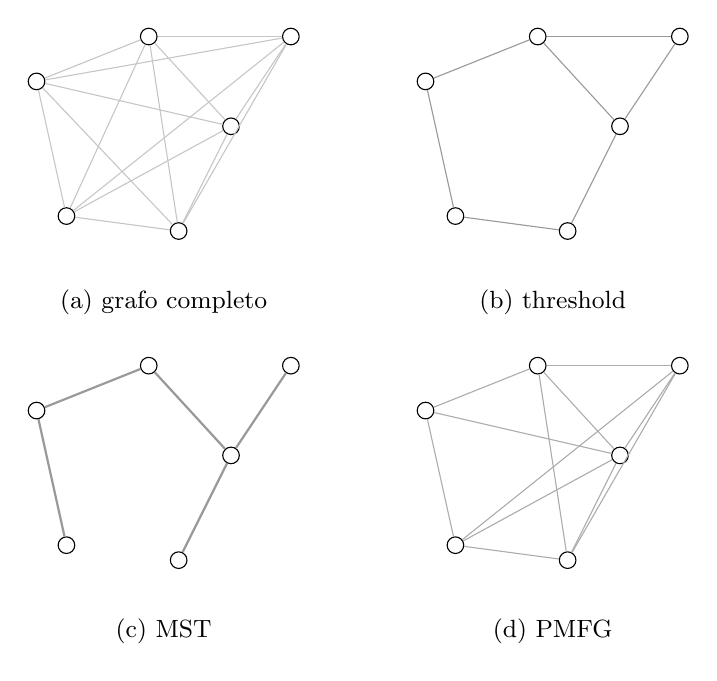
\begin{tikzpicture}[scale=0.95, every node/.style={font=\small},
    nd/.style={circle, draw, fill=white, inner sep=0pt, minimum size=6pt}]
\foreach \s/\dx/\dy/\lab in {0/0/0/{(a) grafo completo}, 1/5.2/0/{(b) threshold}, 2/0/-4.4/{(c) MST}, 3/5.2/-4.4/{(d) PMFG}} {
    \begin{scope}[xshift=\dx cm, yshift=\dy cm]
        \node[nd] (n1\s) at (0.0,2.4) {};
        \node[nd] (n2\s) at (1.5,3.0) {};
        \node[nd] (n3\s) at (2.6,1.8) {};
        \node[nd] (n4\s) at (1.9,0.4) {};
        \node[nd] (n5\s) at (0.4,0.6) {};
        \node[nd] (n6\s) at (3.4,3.0) {};
        \node at (1.7,-0.55) {\lab};
    \end{scope}
}
% (a) completo
\foreach \a/\b in {1/2,1/3,1/4,1/5,1/6,2/3,2/4,2/5,2/6,3/4,3/5,3/6,4/5,4/6,5/6} {
    \draw[gray!45] (n\a0)--(n\b0);
}
% (b) threshold
\foreach \a/\b in {1/2,1/5,2/3,2/6,3/4,3/6,4/5} {
    \draw[gray!80] (n\a1)--(n\b1);
}
% (c) MST
\foreach \a/\b in {1/2,1/5,2/3,3/4,3/6} {
    \draw[gray!80, thick] (n\a2)--(n\b2);
}
% (d) PMFG
\foreach \a/\b in {1/2,1/3,1/5,2/3,2/4,2/6,3/4,3/5,3/6,4/5,4/6,5/6} {
    \draw[gray!65] (n\a3)--(n\b3);
}
\end{tikzpicture}
\caption[Strategie di filtraggio del grafo di correlazione]{Effetto delle strategie di filtraggio sullo stesso insieme di sei nodi. Lo schema è illustrativo e non deriva da dati reali.}
\label{fig:graph-filtering}
\end{figure}

\begin{table}[H]
\centering
\caption[Confronto tra le strategie di costruzione del grafo]{Confronto tra le strategie di filtraggio. $N$ è il numero di asset, $\tau$ la soglia di correlazione, $k$ il numero di vicini mantenuti per nodo.}
\label{tab:graph-construction}
\begin{tabular}{@{}lcccc@{}}
\toprule
\textbf{Strategia} & \textbf{Archi} & \textbf{Parametri} & \textbf{Connessione} & \textbf{Substrato GNN} \\
\midrule
Grafo completo & $N(N-1)/2$ & nessuno & garantita   & inadeguato (denso) \\
Thresholding   & variabile   & $\tau$   & non garantita & adeguato \\
$k$-NN         & $\leq kN$   & $k$      & non garantita & adeguato \\
MST            & $N-1$       & nessuno  & garantita   & povero (albero) \\
PMFG           & $3(N-2)$    & nessuno  & garantita   & adeguato \\
\bottomrule
\end{tabular}
\end{table}

Thresholding e $k$-NN offrono un substrato più adeguato alla GCN, mentre MST e PMFG restituiscono la struttura più informativa dal punto di vista del mercato.

\subsection{Calibrazione della soglia}
\label{sec:tau-calibration}

La pipeline adotta il thresholding sul segno della correlazione: sopravvive l'arco $(i,j)$ se $\rho_{ij}>\tau$, non se $|\rho_{ij}|>\tau$. Una coppia fortemente anticorrelata perde quindi il proprio arco esattamente come una coppia priva di relazione, nonostante il peso di Mantegna corrispondente non sia affatto trascurabile: alla correlazione più bassa osservata nello studio, $\rho=-0{,}551$, l'equazione~\eqref{eq:mantegna-weight} vale ancora $0{,}119$.

La calibrazione (\texttt{calibrate\_tau}) applica il \emph{permutation null} a $24$ finestre di ampiezza $T_w=60$, equispaziate sull'intero periodo campionario. Per ciascuna finestra, \texttt{permutation\_null} genera $B=500$ repliche e ne ricava due campioni di correlazioni: tutte le $\binom{N}{2}=105$ correlazioni di coppia per ogni replica, messe in comune (\emph{pooled}) in un unico campione ($105 \times 500 = 52\,500$ valori), e il solo massimo di correlazione raggiunto all'interno di ciascuna di esse ($B=500$ valori). Il quantile $1-\alpha$ (con $\alpha=0{,}05$) del primo campione rappresenta la stima locale di $\tau$ per quella finestra; lo stesso quantile del secondo campione è invece la stima locale di $\tau_{\mathrm{FWER}}$ — necessariamente più alta, trattandosi del quantile di un massimo su $105$ coppie. Ripetuto su tutte le finestre, il procedimento produce due liste di $24$ stime locali, \texttt{per\_window\_tau} e \texttt{per\_window\_tau\_fwer}, una per soglia. Le $24$ stime locali di ciascuna soglia si riducono infine a un solo valore per l'intero studio prendendone la mediana, non la media, così che una singola finestra anomala non la trascini: $\tau=0{,}2145$, $\tau_{\mathrm{FWER}}=0{,}4311$. Il generatore pseudocasuale che produce le permutazioni è inizializzato con un seme fisso (\texttt{config.seed}): rieseguire la calibrazione restituisce esattamente le stesse soglie. La soglia più severa, $\tau_{\mathrm{FWER}}$, non entra nell'addestramento della GCN: il \cref{ch:topological-evolution} la usa come riferimento per misurare la densità del grafo a un livello di sparsità maggiore.

\begin{listing}[H]
\begin{minted}{python}
def permutation_null(returns_window: np.ndarray | pd.DataFrame, n_permutations: int, rng: np.random.Generator) -> tuple[np.ndarray, np.ndarray]:
    values = np.asarray(returns_window, dtype=np.float64)
    n_obs, n_assets = values.shape
    replicas = np.broadcast_to(values, (n_permutations, n_obs, n_assets))
    shuffled = rng.permuted(replicas, axis=1)
    corr = correlation_from_windows(shuffled.transpose(0, 2, 1))
    rows, cols = np.triu_indices(n_assets, k=1)
    pairs = corr[:, rows, cols]
    return pairs.reshape(-1), pairs.max(axis=1)
\end{minted}
\caption{\texttt{permutation\_null}}
\label{lst:permutation-null}
\end{listing}

\begin{listing}[H]
\begin{minted}{python}
def calibrate_tau(returns: pd.DataFrame, config: Config) -> TauCalibration:
    # Read window, n_windows, alpha, n_permutations from config file
    ...
    n_obs = len(returns)
    starts = np.linspace(0, n_obs - window, n_windows).round().astype(int)
    rng = np.random.default_rng(config.seed)
    quantile = 1.0 - alpha
    per_window_tau: list[float] = []
    per_window_tau_fwer: list[float] = []
    for start in starts:
        window_returns = returns.iloc[start : start + window]
        pooled, max_per_permutation = permutation_null(
            window_returns, threshold_config.n_permutations, rng
        )
        per_window_tau.append(float(np.quantile(pooled, quantile)))
        per_window_tau_fwer.append(float(np.quantile(max_per_permutation, quantile)))
    return TauCalibration(
        tau=float(np.median(per_window_tau)),
        tau_fwer=float(np.median(per_window_tau_fwer)),
        ...
    )
\end{minted}
\caption{\texttt{calibrate\_tau}}
\label{lst:calibrate-tau}
\end{listing}

Applicare $\tau$ o $\tau_{\mathrm{FWER}}$ al tensore delle correlazioni $\{C_t\}$ della \cref{sec:correlation-dependence-pitfalls} equivale a filtrare la matrice dei pesi di Mantegna \texttt{weights} ($W$), indicata d'ora in poi con $W_{\mathrm{full}}$ per distinguerla dalle sue versioni filtrate: la maschera booleana è calcolata sulla correlazione, ma il valore che sopravvive è il peso di Mantegna, non riscalato. Per $\tau^\star\in\{\tau,\tau_{\mathrm{FWER}}\}$,
$$W^\star_{ij} = \begin{cases} W_{\mathrm{full},ij} & \text{se } \rho_{ij}>\tau^\star, \\ 0 & \text{altrimenti}, \end{cases}$$
da cui $W_{\mathrm{thresh}}$ per $\tau^\star=\tau$ e $W_{\mathrm{FWER}}$ per $\tau^\star=\tau_{\mathrm{FWER}}$.

\begin{listing}[H]
\begin{minted}{python}
def apply_threshold(corr: np.ndarray, weights: np.ndarray, tau: float) -> np.ndarray:
    mask = np.asarray(corr, dtype=np.float64) > tau
    return np.where(mask, np.asarray(weights, dtype=np.float64), 0.0)
\end{minted}
\caption{\texttt{apply\_threshold}}
\label{lst:apply-threshold}
\end{listing}

A partire da $W_{\mathrm{thresh}}$, la funzione \texttt{normalized\_adjacency} calcola per ogni finestra l'adiacenza rinormalizzata $\hat A$ dell'equazione~\eqref{eq:renormalization}, con $A=W_{\mathrm{thresh}}$: somma la matrice identità, ricava il grado di ciascun nodo sul grafo così modificato e normalizza simmetricamente (\cref{lst:normalized-adjacency}).

\begin{listing}[H]
\begin{minted}{python}
def normalized_adjacency(weights: np.ndarray, *, self_loops: bool = True) -> np.ndarray:
    weights = np.asarray(weights, dtype=np.float64)
    n_nodes = weights.shape[-1]
    adjacency = weights + np.eye(n_nodes) if self_loops else weights.copy()
    degree = adjacency.sum(axis=-1)
    if (degree <= 0).any():
        raise ValueError(...)
    d_inv_sqrt = degree ** -0.5
    return d_inv_sqrt[..., :, None] * adjacency * d_inv_sqrt[..., None, :]
\end{minted}
\caption{\texttt{normalized\_adjacency}}
\label{lst:normalized-adjacency}
\end{listing}

Si aggiungono i self-loop azzerati in precedenza nel \cref{lst:mantegna-weights}. Con i self-loop attivi il grado di ogni nodo vale almeno $1$ anche quando la soglia lo isola, caso che si presenta per almeno uno degli asset in $62$ delle $1\,947$ finestre. Il controllo sul grado nullo protegge invece l'uso con \texttt{self\_loops=False}, che il \cref{ch:topological-evolution} sfrutta per costruire il Laplaciano normalizzato sul grafo privo di self-loop. Il tensore $\hat A$ che ne risulta è l'input strutturale della GCN nel \cref{ch:training-and-comparison}.

\section{Grafi dinamici e snapshot indipendenti}
\label{sec:dynamic-graphs-temporal-question}

Si dispone ora di una successione $\{G_t\}_t$ di grafi pesati sugli stessi $N=15$ nodi, uno per ciascuna delle $1\,947$ posizioni della finestra mobile. Lo studio tratta tale successione come una serie di \emph{snapshot} indipendenti: il modello è applicato a ciascun $G_t$ separatamente, senza alcun meccanismo che colleghi $G_t$ a $G_{t+1}$. La GCN del \cref{ch:forecasting-models} lo consente perché i suoi parametri agiscono sullo spazio delle feature e non sui nodi. La struttura entra nel calcolo solo attraverso $\hat A$, e lo stesso layer si applica senza modifiche a realizzazioni diverse del grafo. Il \cref{ch:training-and-comparison} utilizza il grafo della finestra che si chiude in $t$ per prevedere $r_{t+1}$ e valuta il modello con un protocollo walk-forward che tratta ogni fold indipendentemente dai precedenti (\cref{sec:tc-walkforward}). Due grafi consecutivi condividono quindi $59$ delle $60$ osservazioni e sono quasi identici (\cref{sec:correlation-dependence-pitfalls}), ma il modello predittivo non sfrutta questa continuità. La successione $\{G_t\}$ è letta come serie temporale solo nel \cref{ch:topological-evolution}, a scopo descrittivo.
